\documentclass{article}

\usepackage[a4paper,margin=2.5cm]{geometry}
\usepackage{graphicx}
\usepackage{amsmath}
\usepackage{amssymb}
\usepackage{listings}
\usepackage{amsthm}
\usepackage{hyperref}
\usepackage{amsfonts}
\usepackage{parskip}
\graphicspath{images}

\newcommand{\code}[1]{\texttt{#1}}

\title{Object Oriented Programming Report}
\author{Giorgio Grigolo}
\date{Semester 1, 2022}

\begin{document}

\maketitle
\begin{abstract}
    \begin{center}
        This report is a documentation of the development of a Java implementation of a Village War Game and a C++ implementation of Minesweeper, 
        which was developed as part of the Object Oriented Programming course at the University of Malta.
    \end{center}

    \begin{center}
        \textbf{Repository: }\href{https://github.com/girogio/oop-games}{https://github.com/girogio/oop-games}\\
        \textbf{Last commit: } 
    \end{center}
\end{abstract}

\tableofcontents

\newpage

\section{Village War Game --- A Java Implementation}

\subsection{Introduction}

My village war game, code-named \code{Clash of Clubs} is an offline multiplayer turn-based strategy game,
where the player is in charge of a village, and must defend it from the attacks of 
the enemy. The player must collect resources in order to build new buildings and upgrade existing ones, through which he can train troops,
collect more resourcse and even attack the enemy.

The game also features an AI with configurable levels difficulty, which can be used to play against.
It will take turns with the player, and will try make a fixed number of actions per turn, 
depending on the difficulty level. Note that the AI is quite smart, meaning that it will not make any invalid choices,
like trying to purchase a building that is too expensive, or train a troop for which no training hut is available.

\subsection{Implementation}

\subsubsection{UML}

For simplicity, the top level UML only contains unidirectional dependencies, aggregations and compositions.
More detailed subsections of this UML will be discussed later, where all the dependencies will be shown.

\vspace{3em}
\begin{figure}[h]
	\centering
	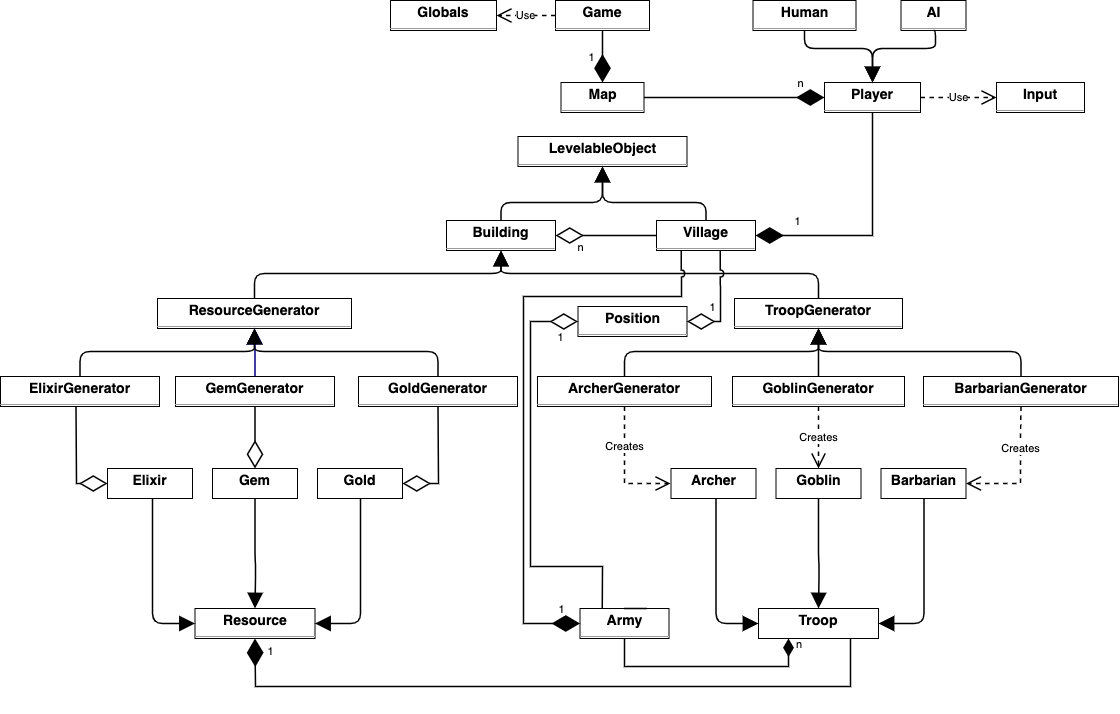
\includegraphics[width=1\textwidth]{images/coc-uml.png}
	\caption{High level UML Diagram}
\end{figure}

\newpage

\subsection{Design Choices}

In view of the fact that the game intrinsically exhibits multiple object oriented design 
patterns, it was noted that the design stage was crucial to the development of the game. Structurally,
the project was split into a number of packages, which are the following:

\begin{itemize}
	
	\item \code{game} --- contains the main class, which is the entry point of the game, and the \code{Game} class, which is the main game loop.
	\item \code{players} --- contains the \code{Player} class, which is the base class for a \code{Player}, and the \code{Human} and \code{AI} classes, which inherit the \code{Player} class. This package also contains the \code{Village} given that its ownership is tied to a single \code{Player}.
	\item \code{buildings} --- contains the \code{Building} class, which is the base class for all buildings, and the respective building type subclasses, namely the \code{ResourceGenerator} and the \code{TroopGenerator} classes.
	\item \code{resources} --- contains the \code{Resources} class, which is the base class for all troops, and the respective troop type subclasses, namely the \code{Gold}, \code{Elixir} and \code{Gem} classes.
	\item \code{troops} --- contains the \code{Troop} class, which is the base class for all troops, and the respective troop type subclasses, namely the \code{Archer}, \code{Goblin} and \code{Barbarian} classes.
	\item \code{utils} --- contains various helper singleton helper classes, to facilitate certain common tasks, as well as any miscellaneous classes that did not fit in the previous packages.
	\item \code{exceptions} --- contains all of the exceptions that could be thrown by any action in the game.
	      
\end{itemize}

In the following pages, I will go through most of the packages, and explain the interactions between them as well as the reasoning behind it.


All of the class methods will be omitted from the following UML as the sheer amount of them makes it unfeasible for them to be displayed neatly.
However, any relevant function will be quoted and briefly explained when needed.


\subsubsection*{Game}

As can be seen in the diagram hereunder, \code{Village}s are owned by
\code{Player}s, and \code{Player}s are the ones that can perform actions that
affect their Villages.

\begin{figure}[h]
	\vspace{1em}
	\centering
	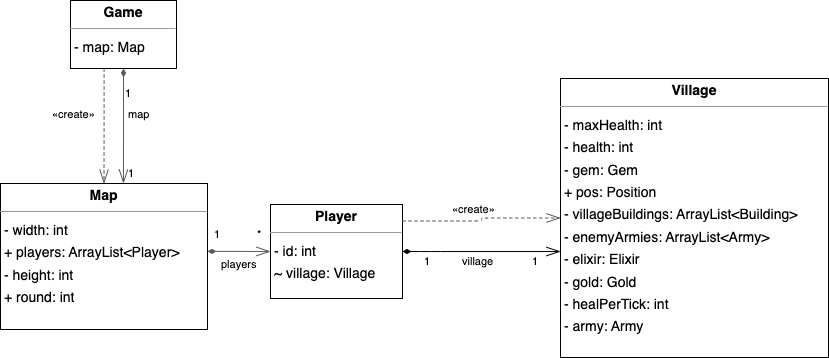
\includegraphics[width=1\textwidth]{images/player-game.png}
	\caption{Game $\leftrightarrow$ Player interactions.}
\end{figure}

The main game loop, called \code{doRound()} will recursively execute itself,
until the win condition has been met. Every round, the following things happen:

\newpage

\begin{enumerate}
	\item Dead players are removed from the \code{players} array in the \code{Map}.
	\item Each \code{Player} will have its \code{doTurn()} method executed.
	\item The win condition check is executed.
	\item Each player's (\code{Village}'s) \code{Army} will march to the set destination.
	\item The round count will be incremented.
\end{enumerate}

\subsubsection*{Player}

We will now define the \code{doTurn()} method in the \code{Player} class, which,
as explained in the previous section, is executed once for every player each
round. 

As per specification, a player's turn consists of the following stages

\begin{enumerate}
	\item Friendly troop arrival --- if the \code{Player}'s \code{Village}'s army has a
	      distance of 0 ticks to cover, and its position is that of the village, we
	      can safely conclude that it's at home, and that therefore each troop must
	      empty their inventory in the appropriate village resource pools.
	\item Enemy troop arrival --- if the \code{Player}'s \code{Village}'s
	      \code{enemyArmies} contains any armies that have no distance to cover, and
	      their position is equal to that of the village, we can safely conclude that these armies 
	      are allowed to attack the \code{Village}. This attack phase will be discussed in more detail later.
	\item Resource Earning --- the \code{Player}'s \code{Village}'s
	      \code{villageBuildings} array will be iterated through, and each
	      \code{Building} will be asked to execute its \code{doTick()} method. For
	      \code{troopGenerators}, this does nothing, as they need to be interacted
	      with voluntarily. If the \code{Building} is a \code{resourceGenerator}, it
	      will generate the appropriate amount of resources, and add them to the
	      \code{Village}'s resource pool accordingly.
	\item Player actions --- according to the player type (\code{Human} or
	      \code{AI}), the appropriate menu loop will be displayed, or the
	      \code{Player} will take a fixed preconfigured number of random actions and pass it's
	      turn. This is defined through overriden methods in the \code{Human}
	      and \code{AI} classes. Furthermore, since we know that a \code{Player}
	      has to be either a \code{Human} or an \code{AI}, we define the
	      \code{playerInput()} method as abstract, to be later implemented in
	      the respective subclasses.
\end{enumerate}


\subsubsection*{Levelable Objects}

Before we introduce the building types, we must first define the root object
that they inherit. Given the similar system that entities must follow when
leveling up, I thought it would be a good idea to define a base class for them,
as they all would have to have a \code{level}, a specific \code{Resource} needed
to level up, and a specific amount of that \code{Resource} needed to level up. 

\begin{figure}[h]
	\vspace{1em}
	\centering
	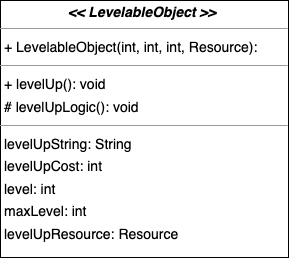
\includegraphics[width=0.3\textwidth]{images/levelableobj.png}
	\caption{\code{LevelableObject} UML}
\end{figure}

The two methods that are defined in the \code{LevelableObject} class, are helper
functions, to make sure that there is enough of the required \code{Resource} to
level up and to actually level up the object. 

However, each \code{LevelableObject} must implement the \code{levelUpLogic()} method, as different attributes 
will change when leveling up, always according to the inherited class type.

\newpage

\subsubsection*{Buildings}

All building types, inherit their main attributes from the \code{Building} super
class, most notably the \code{buildCost} and all the interfaces to implement.

\begin{figure}[h]
	\vspace{1em}
	\centering
	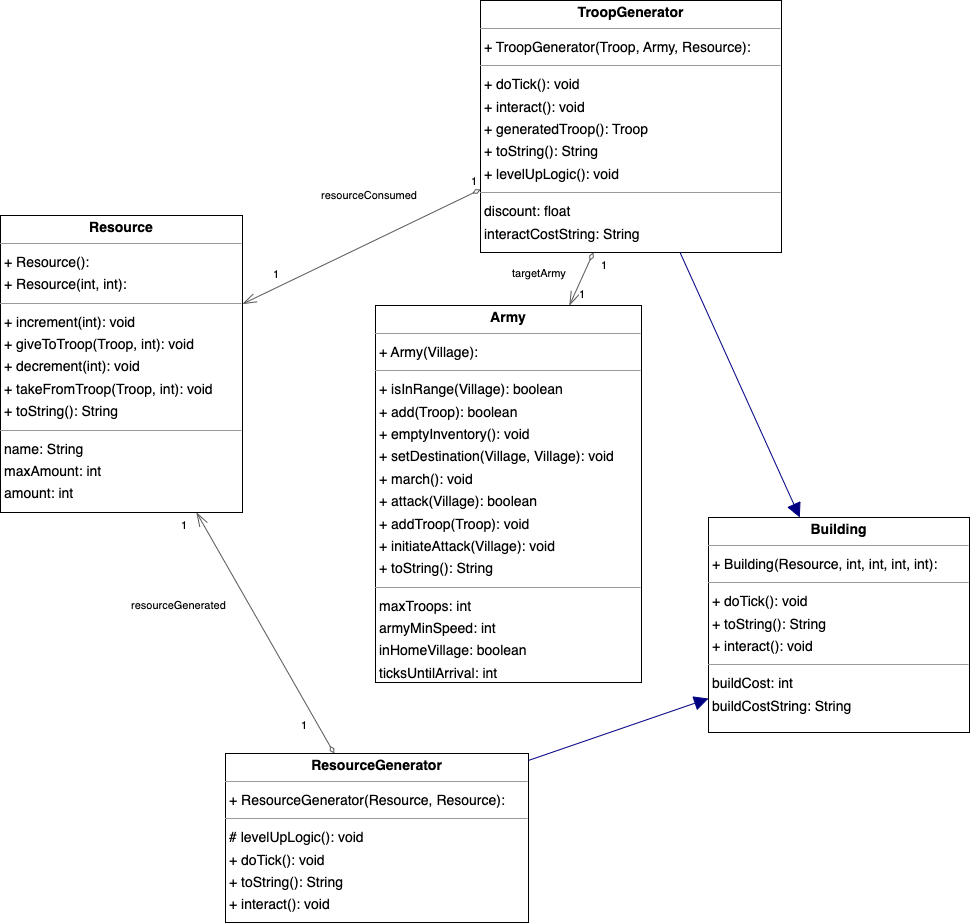
\includegraphics[width=0.9\textwidth]{images/building-uml.png}
	\caption{Building $\leftrightarrow$ Resource interactions.}
\end{figure}

As we can see from the figure above, \code{troopGenerator}s consume a specific
type of \code{Resource} to generate troops, so that they can be assigned to the
\code{targetArmy}. The \code{resourceGenerator}s on the other hand,
generate a specific type of \code{Resource}, which is then transferred to the
\code{Village}'s resource pool.

It should be noted that the Java \code{toString()} method is overriden in each
of the subclasses, to display the appropriate information for each building type
in the user interface.

\newpage

\subsubsection*{Resources}

Given all of the above game-mechanics, we are still missing for a way to
purchase all of the buildings and troops. This is where the \code{Resource}
class as well as it sub-types come into play.

The two construtors in each of the \code{Resource} subclasses, are used to create 
a storage for that specific \code{Resource} type, where the two integer
paramaters define the initial amount of that \code{Resource} type, and the
maximum amount of that \code{Resource} type that can be stored which can be
levelled up (only if it's the \code{Resource} owned by a \code{Village}).

We have seen how we can get some resources from the \code{resourceGenerator}s, but 
we can get more \code{Resource}s by attacking other \code{Village}s, and brought
to us by the \code{Army} that we send to attack.



\begin{figure}[h]
	\vspace{1em}
	\centering
	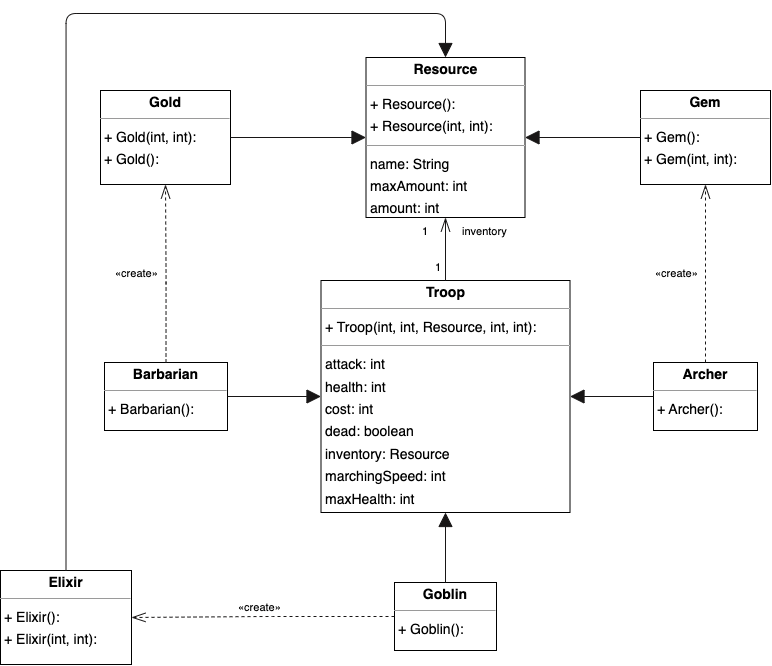
\includegraphics[width=0.9\textwidth]{images/resource-uml.png}
	\caption{Resource $\leftrightarrow$ Building interactions.}
\end{figure}

As can be seen above, each \code{Troop} in the \code{Army} will have an
inventory that is only able to carry a specific type of \code{Resource}. 

\begin{itemize}
	\item \code{Gems} can only be carried by an \code{Archer} and is used to
	      purchase a \code{Goblin},
	\item \code{Elixir} can only be carried by a \code{Goblin} and is used to
	      purchase a \code{Barbarian},
	\item \code{Gold} can only be carried by a \code{Barbarian} and is used to
	      purchase an \code{Archer},
\end{itemize}

\textbf{Note:}  All troops form a resource dependency cycle, as to equally distribute the types of 
\code{Resource}s among expenses thus making the game more balanced.

\newpage

\subsubsection*{Armies}

To be able to attack other \code{Village}s, we need to have an \code{Army}, that is, a collection 
of troops that resides in our \code{Village}. The \code{Army} class extends the native Java
\code{ArrayList} class, overloading some of its core methods, to make sure that the \code{Army}
is always balanced, and that it can only contain a specific number of troops (depending on the level of the \code{Village}).

\begin{figure}[h]
	\vspace{1em}
	\centering
	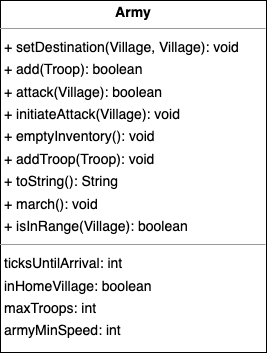
\includegraphics[width=0.25\textwidth]{images/army.png}
	\caption{Army UML Diagram}
\end{figure}

When a user selects the attack option from the menu, they are greeted with a
list of all the other \code{Village}s in the game, and are asked to select one
of them. Once they have selected a \code{Village}, the \code{initiateAttack()}
method is called, which will set the user's \code{Army}'s destination, and add it to 
the target \code{Village}'s encumbent \code{Army} queue.

A variety of helper functions, such as \code{isInRange()} and \code{inHomeVillage()}
are used to quickly determine the position of an \code{Army}.

An attack follows a set of rules, whereby the specifications had to be slightly 
modified to make an attack possible. More particularly, step 3 of the Resolve Combat 
section of the specifications, had to be modified, as killing \code{Troop}s
until the total health of the \code{Troop}s killed is equal to the total attack
of the opposing \code{Army} might result in an infinite loop, in case the amount is not
reached exactly, which is very improbable.

Instead, each \code{Troop} in the attacking \code{Army} will choose one random
defending troop to attack (if any are present) and calls the \code{fight()} \code{Troop} method on it, 
until either the attacking troop is dead, or the defending army is dead.

The \code{fight()} method will bi-directionally deal damage to the two \code{Troop}s, 
and if the defending \code{Troop} is dead, it will be removed from the defending
\code{Army}.

An \code{Army} will stay in the \code{Village} it is attacking, until it is either 
defeated, or it has killed all of the \code{Troop}s in the defending
\code{Army}, at which point it will steal all of the \code{Resource}s from the
\code{Village} it is attacking, and start its trip back to its home \code{Village}. 
This game mechanic is used to make sure that the game is not too easy, and that
the player has to be careful when attacking other \code{Village}s as it leaves them
vulnerable to attacks from other players.
 

\subsubsection*{Position}
The \code{Position} object is given to those entities that are expected to be
able to move around the game map. In essence, the \code{Position} object is a wrapper around a pair of
integers, that represent the x and y coordinates of the entity on the game map. This allows 
us to override the \code{equals()} method, and compare two \code{Position}s
by their coordinates, instead of their memory addresses.

Furthermore, the \code{Position} object has a \code{distance(Position p)} that calculates 
the distance between two \code{Position}s, taking into account the grid-like structure of the map.
In fact, this distance is defined over the taxi-cab metric, which is equivalent to $$ d(p_0, p_1) = |x_1 - x_0| + |y_1 - y_0| $$

\subsubsection*{Exceptions}

Of course, a \code{Human} makes mistakes, and therefore so does our code. To make sure that 
our code is as robust as possible, we have implemented a variety of custom exceptions, that are thrown
when an error occurs. These exceptions are then caught by the \code{Player} class, which displays nicely 
formatted error messages to the user, and allows them to try again the action they were trying to perform.

In this game, the following exceptions are thrown:

    \begin{itemize}
        \item \code{ArmyAwayException} is thrown when the user tries to perform an action on an \code{Army} that is not in their \code{Village}.
        \item \code{ArmyEmptyException} is thrown when the user tries to send an empty \code{Army} to attack.
        \item \code{ArmyFullException} is thrown when the user tries to add a \code{Troop} to an \code{Army} that is already full.
        \item \code{InsufficientResourcesException} is thrown when the user tries to perform an action that requires more \code{Resource}s than they have.
        \item \code{MaxLevelException} is thrown by a \code{LevelableObject} when the user tries to upgrade it to a level that is higher than the maximum level.

    \end{itemize}

\subsubsection*{Globals}

In order to allow maximum flexibility, we have implemented a \code{Globals} class, that contains
all the constants that are used throughout the game. This allows us to easily change the values of
these constants, without having to search through the code for all the places where they are used.

The statically loaded variables in the \code{Globals} class, define the default values of a myriad of
properties of objects. Since I am not a game designer, I did not have the time to come up with balanced 
values for these properties, and therefore I have decided to make them configurable, so that they can be
tweaked by the user.


\newpage

\subsection{Testing}

Due to the sheer number of interactions and possible states that the game can be in, it is very difficult
to test the game manually. Therefore, we have decided to implement a series of automated unit tests, that
test the functionality various parts of the game in an isolated manner, without having to go through all the game menus.

These can be found in the \code{tests} directory under the main package, and are written using the
\code{JUnit} framework. Most notably, the \code{Village}, \code{Army}, and
\code{Resource} interactions were the most crucial to the successful execution
of the game.

The codebase has also been analysed using \code{CodeMR}
\footnote{http://codemr.sourceforge.net/}, which is a static analysis tool for
Java code. With it, we are able to deduce some of the metrics of the quality of the software,
such as the coupling of classes (lower is better), cohesion (higher is better), and complexity.

\begin{figure}[h]
    \centering
    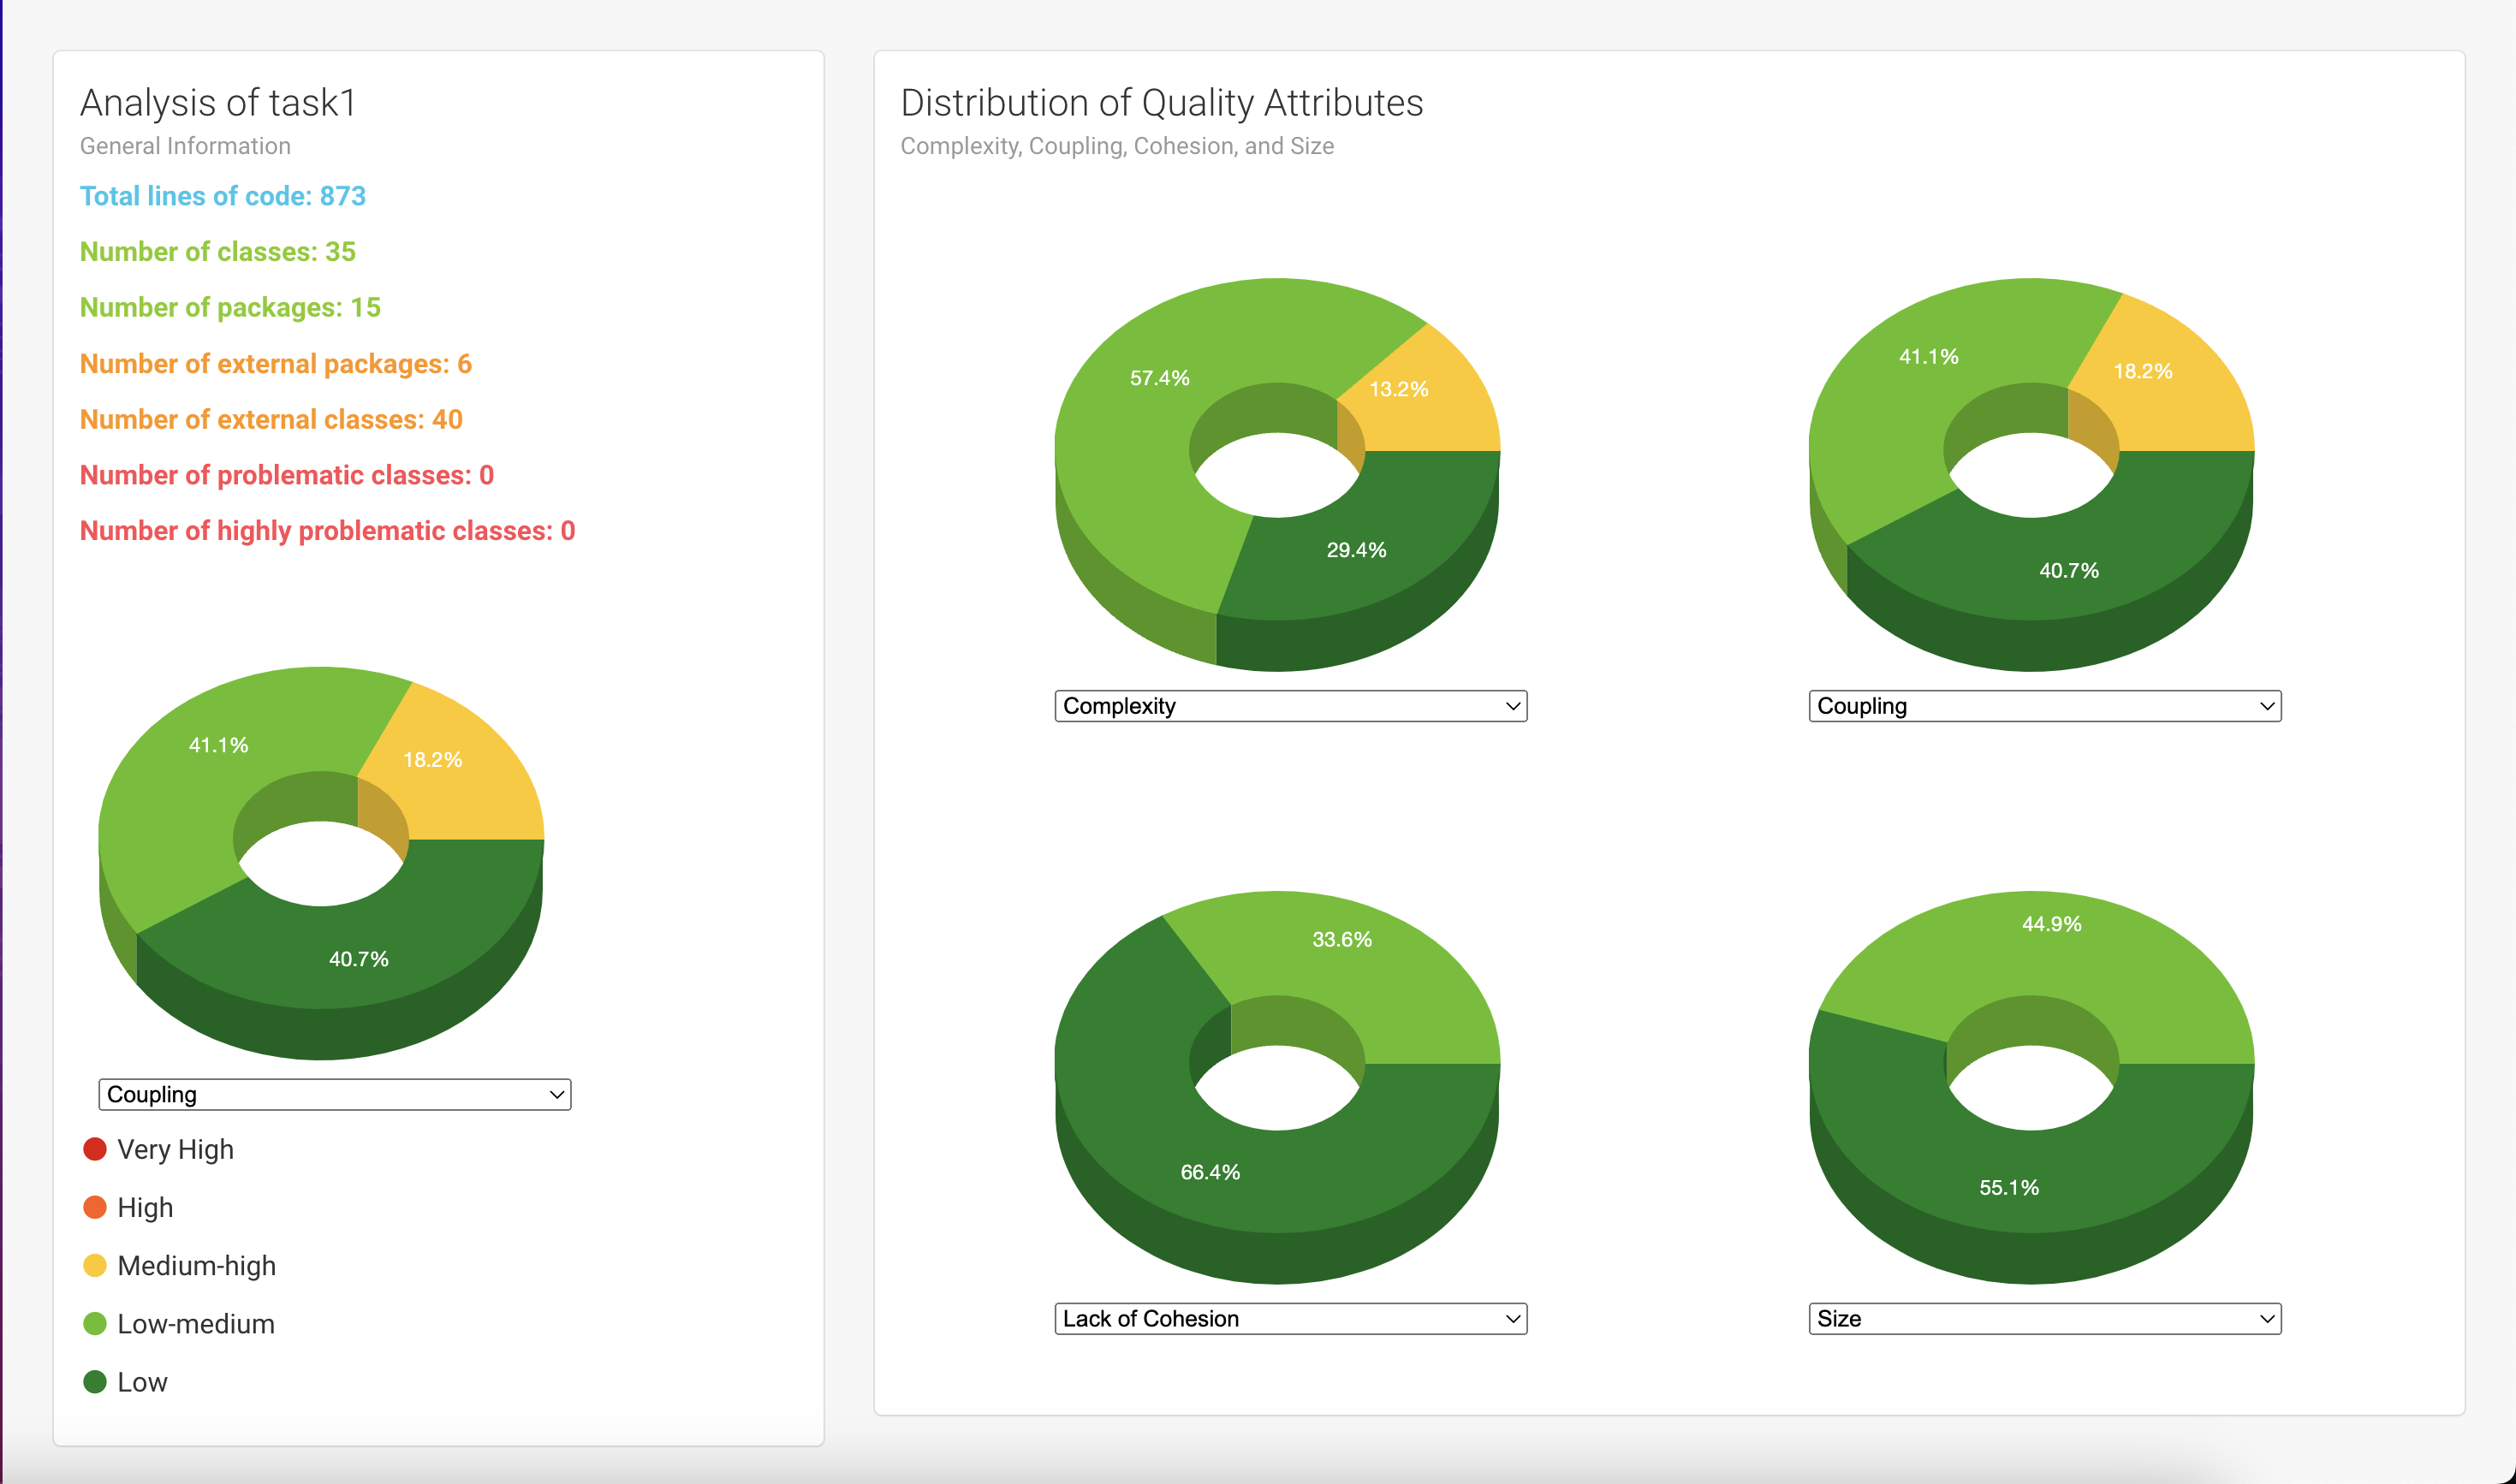
\includegraphics[width=0.9\textwidth]{images/code_mr.png}
    \caption{CodeMR results}
    \label{fig:codemr}
\end{figure}


\subsection{Critical Evaluation and Limitations}

There are a lot of avenues that could have been improved, for the sake of the
expansion of the game. For example, to create a new \code{Troop}, a developer must create
a new class for every new \code{Troop} type, and also add a new \code{TroopGenerator}. This could have been 
fixed by using a \code{Factory} design pattern, and creating a \code{TroopFactory} that would
create \code{Troop}s, say, based on a string identifier.

Another limitation of the game is that it is not possible to save the game state, and
resume it at a later time. This could have been implemented by serializing the game state
to a file, and then deserializing it when the game is loaded.

Furthermore, there is a possibility that \code{Village}s can spawn really close to each other,
making the game uninteresting, as an \code{Army} would arrive in one turn.

The specifications were also followed quite closely, except for the combat resolution algorithm.


\newpage

\section{Minesweeper --- A C++ Implementation}

\subsection{Introduction}
Minesweeper is a logic puzzle video game genre generally played on personal
computers. The game features a grid of clickable squares, with hidden ``mines''
scattered throughout the board. The objective is to clear the board without
detonating any mines, with help from clues about the number of neighboring
mines in each field.
In this section (\thesection), we will implement Minesweeper with the help of
ncurses\footnote{Ncurses is a programming library providing an application with a 
	terminal-independent screen-painting and keyboard-handling facility in a
text-mode environment.} and C++.

The game is played on a board of tiles, each of which is either a mine or
empty. The player is initially presented with a board of tiles, and
must use logic to deduce the locations of the mines. The player can click on a
tile to reveal it. If the tile is a mine, the player loses. If the tile is
empty, the tile will be revealed, and if it has no neighboring mines, all of
its neighboring tiles will be revealed as well. If the tile has neighboring
mines, the number of neighboring mines will be displayed on the tile. If the player
marks all of the mines, the player wins.


\subsection{Implementation}

\subsubsection{UML}

\vspace{6em}
\begin{figure}[h]
	\centering
	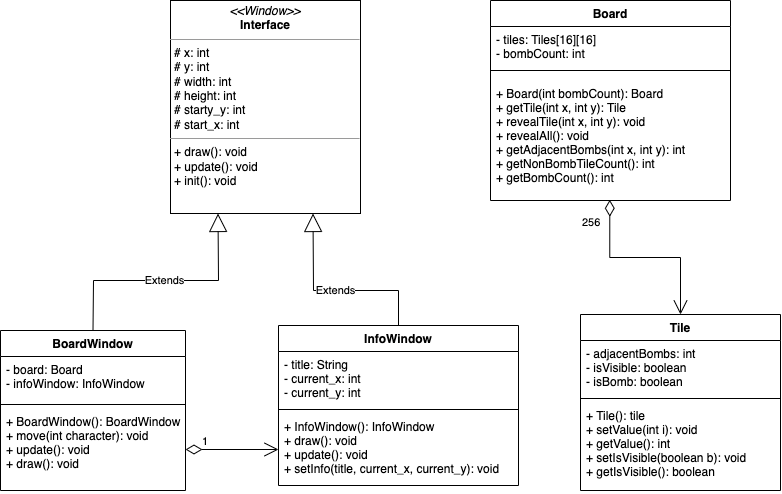
\includegraphics[width=0.9\textwidth]{images/minesweeper.png}
	\caption{Minesweeper UML Diagram}
\end{figure}

\newpage

\subsection{Design Choices}

The user interface, to be preferably displayed on a full screen terminal, is
usable through the traditional `\code{wasd}' keys, or the vim\footnote{Vim is a free and open-source, screen-based text editor.}-oriented `\code{hjkl}' keys, and the `\code{Space}'
key to reveal a tile.

The user interface uses the ncurses library. Being by far the most
difficult part of this program that I had to implement, it was the one that required most of 
my attention and time. Even though it originated in the form of a C library, I have created
an abstract handler class \code{Window}, in such a way that I thought would best fit the
needs of this program. The window class is inherited by the two windows that are shown
to the user: the \code{BoardWindow} and the \code{InfoWindow}.

The \code{BoardWindow} will tile by tile, get the properties of the tile, and
display them accordingly; either hidden or revealed. In case of the latter, the number 
of adjacent mines will be shown, in an appropriate color. The \code{InfoWindow} will display the current selected coordinates, mostly for debugging
purposes. When the game is over be it won or lost, it will display the final message respectively.

Of course, each window type update and draw methods are different, as they have different
properties to display. Whilst inheriting a common interface, they are still
different classes.

As for the board, it made sense for it to act as a storage for the tiles, as well as a 
handler for the different tile states. One could say that the \code{Board} is a list-like data structure, 
with utility functions modifying the internal state for every atomic object inside of it, the \code{Tile}.

A \code{Tile} is just a POCO (a plain old C++ object), which means that the
class only contains privated class variables, together with their public 
getters and setters, thus making it encapsulated and low-coupled.


\subsection{Testing}

The game, being simple in nature, is easy to test. I have tested
the \code{Board} class by creating a board with a given number of mines, and
then checking if the number of mines is correct. I have also tested the
\code{Board} class by checking if the number of adjacent mines is correct.

This was done through manual inspection, together with a hidden keybind set to `\code{C}' that would reveal all the tiles.
A second debug keybind was set to `\code{B}' which would turn the currently selected tile into a mine, 
to see that the adjacent mines were correctly calculated.

The win condition was tested by generating a board with all mines except for one tile, and clicking on it
which is known to us given the \code{revealAll} function, which is called when `\code{C}' is pressed.

A lot of care has been put in such a way that on quitting, (keybind: `\code{Q}'), the windows are destroyed 
through the pipeline provided by ncurses \code{endwin()}, as to reduce as many memory leaks as possible.

\subsection{Critical Evaluation and Limitations}

The game is fully functional, and it is playable. It is also easy to use, and
it is very intuitive. The game was developed with scalability in mind, and one can set 
the board size and the number of mines in the \code{Board} class.

However, the game is not perfect, and it has some limitations. One of these is the fact that
user interface is not resizable, and it will look unplayable on a terminal smaller than
29x102 characters.

Also, since the mines are randomly generated, the game can be lost in the first move, which is not the way 
the original minesweeper works. The original minesweeper would randomly seed the board mine position randomization process
after the first move, in such a way that your first move is never a mine.

\newpage



\end{document}